% !TEX TS-program = xelatex
% !TEX encoding = UTF-8 Unicode
% !Mode:: "TeX:UTF-8"
\documentclass{resume}
%\documentclass[8pt]{article}
%\usepackage{zh_CN-Adobefonts_external} % Simplified Chinese Support using external fonts (./fonts/zh_CN-Adobe/)
\usepackage{zh_CN-Adobefonts_internal} % Simplified Chinese Support using system fonts
\usepackage{linespacing_fix} % disable extra space before next section
\usepackage{cite}
\usepackage[colorlinks,linkcolor=blue,anchorcolor=blue,citecolor=green,urlcolor=blue]{hyperref}
\usepackage{amssymb}
\usepackage{amsmath}
\usepackage{color}
% \definecolor{usercolor}{rgb}{0.5,0.8.0.7}
%for header image
\usepackage{graphicx}
\usepackage{tikz} %用于定位照片
\usetikzlibrary{calc}
%for floating figures
\usepackage{wrapfig}
\usepackage{float}
\usepackage{enumitem} % 控制列表格式和缩进等等
%\floatstyle{boxed}
%\restylefloat{figure}
\usepackage{geometry}
\geometry{left=1.5cm,right=1.5cm,top=0.8cm,bottom=0.1cm}
% \setstretch{1.25}
% \newcommand{\vcenteredinclude}[1]{\begingroup
% \setbox0=\hbox{\hspace*{-0.1cm}\includegraphics[width=0.1cm]{#1}}%
% \parbox{\wd0}{\box0}\endgroup}


\begin{document}
\pagenumbering{gobble} % suppress displaying page number

\name{ 张\hspace{0.1cm}贵\hspace{0.1cm}瑞 }

% {E-mail}{mobilephone}{homepage}
% be careful of _ in emaill address
{\centerline{\contactInfo{17781444956@163.com}{177-8144-4956}{1997-02-23}}}
{\qquad \qquad \qquad \qquad \qquad
{GitHub:\href{https://github.com/freesix}{https://github.com/freesix}}\quad
个人博客:\href{https://freesix.github.io/}{freesix.github.io}}

\begin{tikzpicture}[remember picture,overlay]
  \node[anchor = north east] at ($(current page.north east)+(-2cm,-1.2cm)$){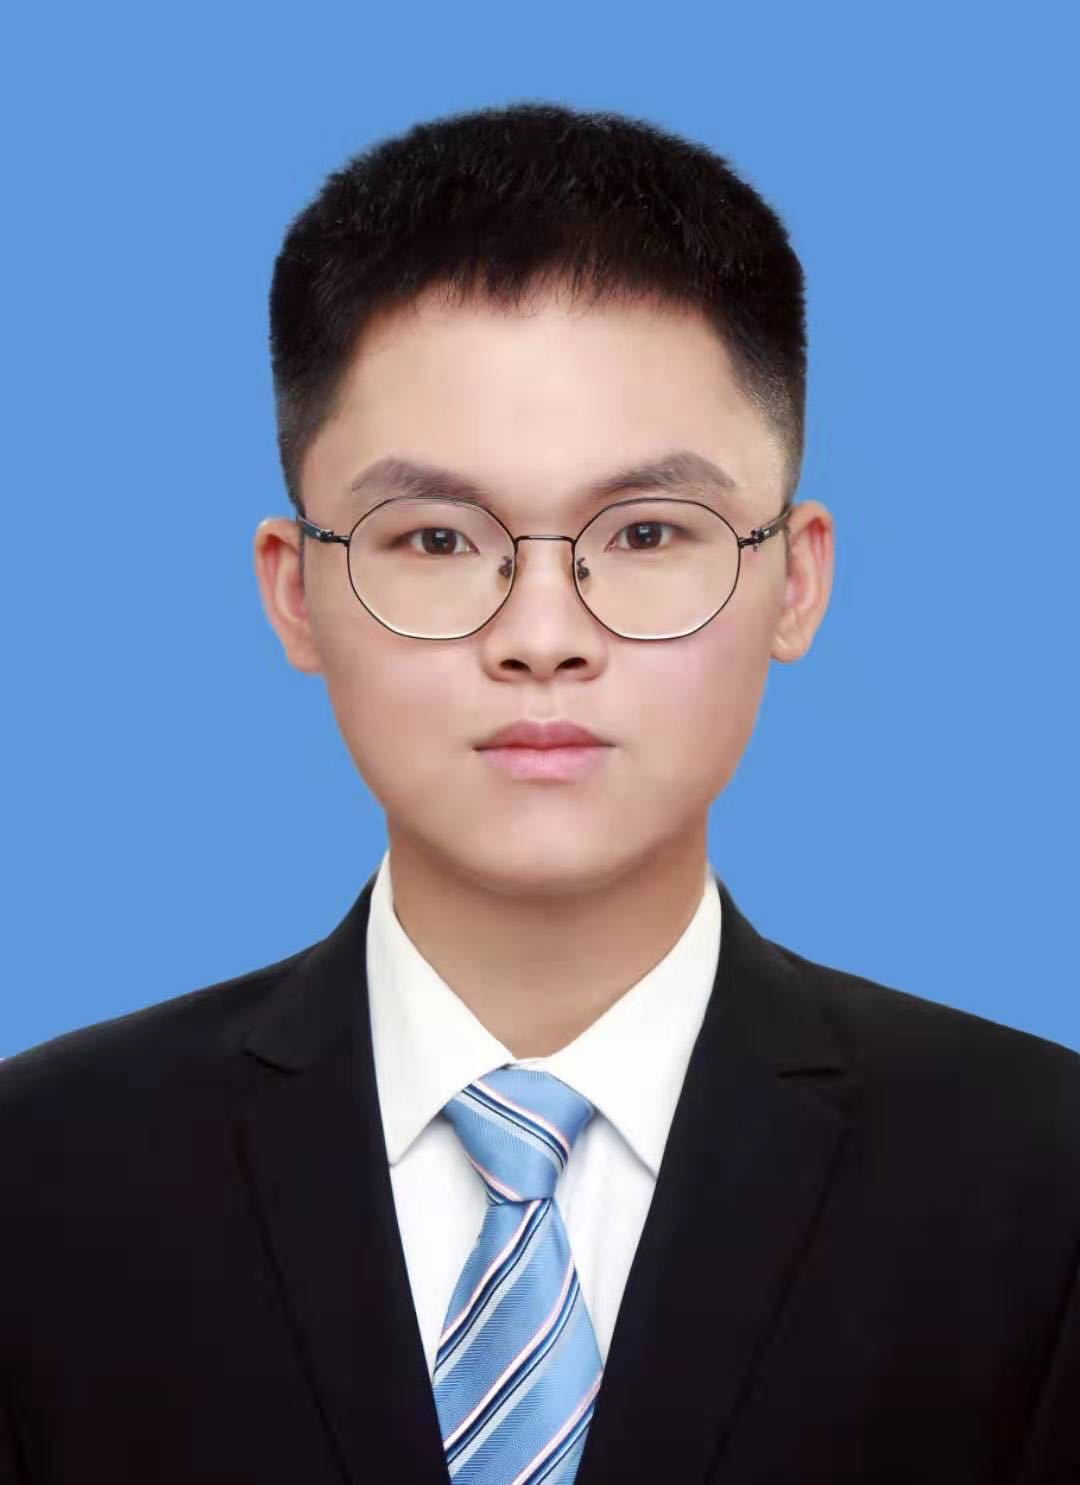
\includegraphics[width=2.5cm]{images/照片.jpg}};
\end{tikzpicture}
% \centerline{\includegraphics[width=0.2cm]{imazhen.jpg}}

% {E-mail}{mobilephone}
% keep the last empty braces!
%\contactInfo{xxx@yuanbin.me}{(+86) 131-221-87xxx}{}
求职意向:\textbf{SLAM算法工程师、3D算法工程师等}
\section{\textcolor[RGB]{50,50,190}{\faBriefcase 工作 / 实习经历}}

\datedsubsection{\textbf{FAE工程师}-总经理室\qquad 上海芯圣电子股份有限公司}{2020年5月 -- 2021年8月(1年3个月)}
\begin{itemize}
  \item 产品的应用开发,编写芯片例程、设计demo板。便携式血氧仪和公司触摸控制板的算法优化和改进。
  \item 负责对客户工程师的技术培训,协助客户工程人员在方案中导芯片。
  % \item 发挥FAE的技术能力和经验,协助客户工程人员在方案中导入芯片。
  % \item 嵌入式软件开发,如血氧仪、触摸控制板、锂电充手电等消费类电子产品开发。
    % \item 负责客户技术人员的技术培训,帮助其提高对产品的认知,培养对我方产品的使用习惯。
  % \item 收集客户需求和产品反馈,协助产品部门和推动产品的改进。
  \item 负责华东片区大客户,如鱼跃医疗、科大讯飞、小米等公司的现场技术支持。
  % \item 内部营销人员、新员工的技术培训,围绕本公司产品撰写对外教材和录制培训视频。
\end{itemize}

\datedsubsection{\textbf{3D算法工程师}-AI技术部\quad 第六镜科技有限公司(实习)}{2023年11月 -- 2024年2月(4个月)}
% 3D算法工程师\qquad \qquad \quad AI技术部
\begin{itemize}
  \item 负责铁轨轮廓结构光3D重建项目的光条中心线提取、点云处理部分算法。
  \item 改进steger算法,适应高速采集工况下的应用。
\end{itemize}

\datedsubsection{\textbf{SLAM算法工程师}-算法事业部\qquad 四川省寰宇众恒科技有限公司}{2024年2月 -- 至今(7个月)}
\begin{itemize}
    \item 单目惯性SLAM算法的方案调研与移动端适配。解决算法落地过程中产生的各类问题。
    \item 相机内参、IMU参数的单独标定及联合外参标定。
    \item GPS信号在算法中的融入及拒止情况下的轨迹对齐。
\end{itemize}



\section{\textcolor[RGB]{50,50,190}{\faUsers\ 科研 / 项目经历}}

% \end{itemize}


\datedsubsection{\textbf{智慧园区行人跟踪定位}}{2024年2月 -- 至今}
% \begin{description} [leftmargin=60pt]
% \item[\textbf{\textcolor[RGB]{80,100,190}{项目简介:}}]
\textbf{\textcolor[RGB]{80,100,190}{项目简介:}}

\hspace{20pt} 在智能头盔和手机上,利用视觉SLAM算法对工业园区或化工厂房的活动人员进行定位。

\textbf{\textcolor[RGB]{80,100,190}{工作内容:}} 

\hspace{20pt} 1.负责开发基于VINS-FUSION的移动端视觉SLAM定位系统,确保系统能够精确地在智能头盔和手机
上对工业园区或化工厂房内的活动人员进行实时定位。

\hspace{20pt} 2.针对算法设计中遇到的复杂问题进行深入分析和解决,包括但不限于图像畸变矫正、轨迹优化、
边缘化等关键技术环节。

\hspace{20pt} 3.执行相机与惯性测量单元(IMU)的精确标定工作,以提高系统的整体定位精度和稳定性。 

\hspace{20pt} 4.对VINS前端进行必要的修改和优化,增强系统对动态环境变化的适应能力,确保在复杂场景下的定位准确性。

\hspace{20pt} 5.通过持续的系统测试与性能评估,不断迭代改进算法,以满足工业园区高动态、高精度的定位需求
% 实现基于VINS-FUSION的移动端视觉SLAM定位系统。解决出现的轨迹漂移、动态物体、场景退化等问题。相机与IMU的内参外参标定。
% 图像的畸变矫正和VINS前端修改。

% \item[\textbf{\textcolor[RGB]{80,100,190}{工作成果:}}]
\textbf{\textcolor[RGB]{80,100,190}{工作成果:}}

\hspace{20pt} 顺利完成整个开发流程,保证算法在室内室外环境中稳定运行。室内GPS信号退化情况下的轨迹对齐算法融入。


\datedsubsection{\textbf{多视角图像拼接补全算法设计}}{2022年12月 -- 2024年3月}
% \begin{description}[leftmargin=60pt]
% \item[\textbf{\textcolor[RGB]{80,100,190}{项目链接}}:]\hyperlink{https://github.com/freesix/GNN-martch}
% {https://github.com/freesix/GNN-martch}
\textbf{\textcolor[RGB]{80,100,190}{项目链接}}:\hyperlink{https://github.com/freesix/GNN-martch}
{https://github.com/freesix/GNN-martch}

% \item[\textbf{\textcolor[RGB]{80,100,190}{项目简介:}}]
\textbf{\textcolor[RGB]{80,100,190}{项目简介:}}

\hspace{20pt} 将曲面上16块CMOS芯片所成图像拼接成一幅完整的图像。\textbf{图像配准先进算法的研究和实现}。

\textbf{\textcolor[RGB]{80,100,190}{工作内容:}}

\hspace{20pt} 设计先进\textbf{图匹配算法}用于\textbf{图像拼接的特征点配准步骤},借助GNN、极大团匹配、
因子图分解等方法提升配准的精度和鲁棒性,提高对图像特征点离群值的筛选。
% 根据横向项目的需求制定技术路线,撰写需求分析、技术目标等文档,整体拼接算法路线制定,图像匹配
% 部分算法的研究和实现、深度模型的设计和训练等。后续估计失焦图像的PSF用于模糊图像恢复,对畸变
% 图像设计畸变模型估计畸变参数。

% \item[\textbf{\textcolor[RGB]{80,100,190}{工作成果:}}]
\textbf{\textcolor[RGB]{80,100,190}{工作成果:}}
% 论文$\ll$ Image Stitching with Weight Learnable Graph Matching Network$\gg$(暂定),
% 图像配准的性能远高于传统KNN+RANSAC算法或SuperGlue等学习方法。

\hspace{20pt} 提出了一种权重可学习的图注意力机制用于图像拼接的配准步骤,图像配准的性能优于传统的KNN+RANSAC
算法或SuperGlue等学习方法。
% \end{description}
\section{\textcolor[RGB]{50,50,190}{\faCogs\ 技能}}
% increase linespacing [parsep=0.5ex]
\begin{itemize}[parsep=0.5ex]
  \item C/C++、Python、ROS2、Linux、Pytorch
  \item 熟悉VINS-Mono、LIO-SAM,了解Point-LIO、ORB\_SLAM3等框架
  \item 了解IMU预积分、边缘化、极几何、EKF、ESEKF等概念或算法
  \item 对GNN和图匹配相关算法有一定了解,并用于点云配准的研究
  % \item 

\end{itemize}


\section{\textcolor[RGB]{50,50,190}{\faGraduationCap 教育背景}}
\datedsubsection{\textbf{西南民族大学}, 电气工程学院}{2021年9月 -- 2024年6月}
\textit{硕士}\ \ 电子信息专业 \qquad \qquad
\textcolor[RGB]{80,100,190}{\textbf{研究方向}}:
SLAM、图像拼接、点云配准


\datedsubsection{\textbf{上海工程技术大学}, 电气工程学院}{2016年9月 -- 2020年7月}
\textit{学士}\ \ 自动化专业


% \datedsubsection{\textbf{西南民族大学}, 电气工程学院\qquad \qquad \textit{硕士}\ \ 电子信息专业} {2021年9月 -- 2024年6月}
%
% \textcolor[RGB]{80,100,190}{\textbf{研究方向}}:
% SLAM、图像拼接、点云配准
%
% \datedsubsection{\textbf{上海工程技术大学}, 电气工程学院 \qquad \qquad \textit{学士}\ \ 自动化专业}{2016年9月 -- 2020年7月}

\section{\textcolor[RGB]{50,50,190}{\faPaperPlane\ 获奖和科研成果}}
% \begin{itemize}
研究生奖学金两次、本科生奖学金一次、本科校三等奖一次

论文$\ll$ Image Stitching with Weight Learnable Graph Matching Network$\gg$在投
% \end{itemize}
% \end{itemize\i\}
\section{\textcolor[RGB]{50,50,190}{\faChild\ 自我评价}}
拥有良好的自我驱动力,学习能力强,对激光slam、视觉slam、嵌入式软件开发、图像拼
接等领域均有不同程度的涉猎和研究。在以往工作中表现出了组织和团队领导能力,一年多工作时间已成
为区域负责人。


%% Reference
%\newpage
%\bibliographystyle{IEEETran}
%\bibliography{mycite}
\end{document}
